\begin{figure*}[t]
\centering
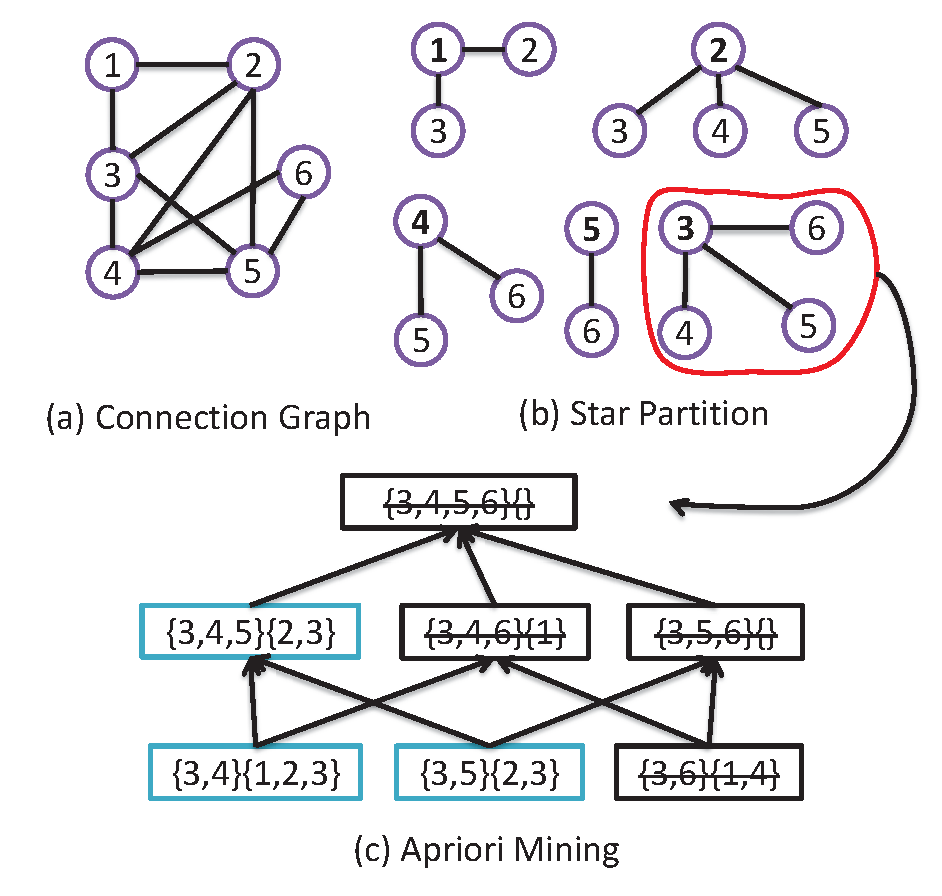
\includegraphics[width=0.8\textwidth]{spm.eps}
%\vspace{-0.5em}
\caption{Star Partitioning and ApRiori Enumerator (SPARE). (a) Aggregated graph $G_A$ generated from Figure 1. (b) Five star partitions are generated from $G_A$. Star IDs are circled, vertexes and inverted lists are in the connected tables.
(c) Apriori Enumerator with various pruning techniques.}
\label{fig:star_partition}
%\vspace{-0.5em}
\end{figure*}

\section{SPARE: Star Partitioning and \\ Apriori Enumerator}
\label{sec:spm}
The aforementioned TRPM scheme replicates snapshots based on the temporal dimension which suffers from two drawbacks. First, the replication factor $\eta$ can be large. Second, the same valid pattern may be redundantly discovered from different partitions.
%which results in redundant works.
To resolve these limitations,
we propose a new Star Partitioning and ApRiori Enumerator, named SPARE, 
to replace the second stage of the mapreduce jobs in Figure~\ref{fig:trm}. 
Our new parallel mining framework is shown in Figure~\ref{fig:star_partition}. 
Its input is the set of clusters generated in each snapshot and the output 
contains all the valid GCMPs. In the following, we explain the two major components: 
star partitioning and apriori enumerator.


\subsection{Star Partitioning}
Let $G_t$ be a graph for snapshot $S_t$, in which each node 
is a moving object and two objects are connected if they appear 
in the same cluster. It is obvious that $G_t$ consists of a set of small cliques. 
Based on $G_t$, we define an aggregated graph $G_A$ to summarize the 
cluster relationship among all the snapshots. In $G_A$, two objects
form an edge if they are connected in any $G_t$s. Furthermore, 
we attach an inverted list for each edge, 
storing the associated timestamps in which the two objects are connected. 
An example of $G_A$, built on the trajectory database in Figure~\ref{fig:related_work}, 
is shown in Figure~\ref{fig:star_partition} (a). 
As long as two objects are clustered in any timestamps, they are connected in $G_A$. 
The object pair $\langle o_1,o_2 \rangle$ appears in two clusters at timestamps 
$2$ and $3$ and is thus associated with an inverted list $(2,3)$.

We use \emph{star}~\cite{yoo2006joinless} as the data structure to capture the pair relationships. 
To avoid duplication, as $G_t$ is an undirected graph and an edge may appear in multiple stars, 
we enforce a global vertex ordering among the objects and propose a concept named \textit{directed star}.

\begin{definition}[Directed Star]
Given a vertex with global ID $s$, its directed star $Sr_s$ is defined as the set of neighboring vertexes with global ID $t>s$. We call $s$ the star ID.
\end{definition}

With the global vertex ordering, we can guarantee that each edge is contained in a unique star partition. Given the aggregated graph $G_A$  in Figure~\ref{fig:star_partition} (a), we enumerate all the possible directed stars in Figure~\ref{fig:star_partition} (b). These stars are emitted from mappers to different reducers. The key is the star ID and the value is the neighbors in the star as well as the associated inverted lists. 
The reducer will then call the Apriori-based algorithm to enumerate all the valid GCMPs.


Before we introduce the Apriori Enumerator, we are interested to 
examine the issue of global vertex ordering.
% on the moving objects.
This is because assigning different IDs to the objects will produce 
different star partitioning results, which will eventually affect the workload 
balance among reducers. The job with the performance bottleneck is often known as a  \emph{straggler}~\cite{kwon2012skewtune}. In the context of star partitioning, a straggler refers to the job assigned with the maximum star partition. We use $\Gamma$ to denote the size of such straggler partition and $\Gamma$ is set to the number of edges in a directed star\footnote{A star is essentially a tree structure and the number of nodes equals the number of edges minus one.}. Clearly, a star partitioning with small $\Gamma$ is preferred. For example, Figure~\ref{fig:star-alt} gives two star partitioning results under 
different vertex ordering on the same graph. The top one has $\Gamma = 5$ while the bottom one has $\Gamma = 3$. Obviously, the bottom one with smaller $\Gamma$ is much more balanced.

\begin{figure}[h]
\centering
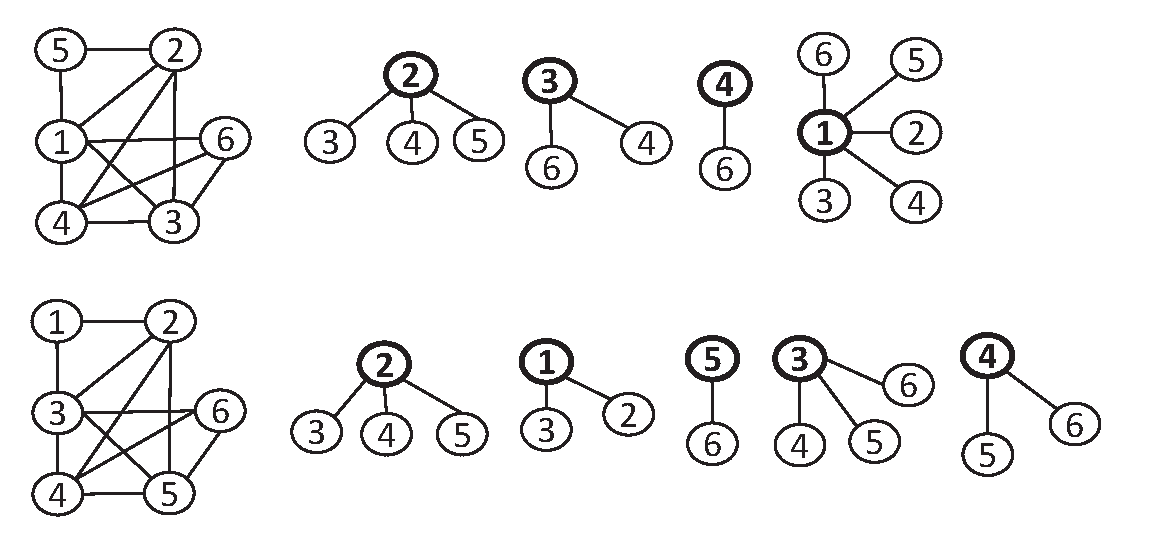
\includegraphics[width=0.35\textwidth]{star-alt.eps}
\caption{Star partitioning with different vertex orderings.}
\label{fig:star-alt}
\end{figure}

Although it is very challenging to find the optimal vertex ordering from the $n!$ possibilities, we observe that a random order can actually achieve satisfactory performance based on the following theorem.


\begin{theorem}
\label{THM:SPM_LB}
Let $\Gamma^*$ be the value derived from the optimal vertex ordering and  $\Gamma$ be the value derived from a random vertex ordering. With probability $1-1/n$, we have $\Gamma = \Gamma^* + O(\sqrt{n \log n})$.
\end{theorem}
\begin{proof}
%\vspace{-0.5em}
See Appendix~\ref{apx:thm2proof}.
\end{proof}
If $G_A$ is dense, we can get a tighter bound for $(\Gamma - \Gamma^*)$.
\begin{theorem}
\label{THM:SPM_LB_INC}
Let $d$ be the average degree in $G_A$. If $d\geq \sqrt{12\log n}$, with
high probability $1-1/n$, $\Gamma = \Gamma^* + O(\sqrt{d\log n})$.
\end{theorem}
\begin{proof}
%\vspace{-0.5em}
See Appendix~\ref{apx:thm2proof}.
\end{proof}
Hence, we can simply use object ID to determine the vertex ordering in our implementation.


\subsection{Apriori Enumerator}
Intuitively, given a GCMP with an object set $\{o_1,\ldots,o_m\}$, 
all the pairs of $\langle o_i,o_j \rangle$ with $1\leq i<j\leq m$ must 
be connected in the associated temporal graphs $\{G_t\}$. This inspires us to leverage the classic Apriori algorithm~\cite{agrawal1994fast} to enumerate all the valid GCMPs starting from pairs of objects. However, we observe that the monotonicity property does not hold between an object set and its supersets.

\begin{example}
In this example, we show that if an object set is not a valid pattern, we cannot prune all its super sets.
Consider two candidates $P_1=\langle o_1,o_2:1,2,3,6 \rangle$ and $P_2=\langle o_1,o_3:1,2,3,7 \rangle$. 
Let $L=2,K=3$ and $G=2$. Both candidates are not valid patterns because the constraint on $L$ is not satisfied. 
However, when considering their object superset $\langle o_1,o_2,o_3 \rangle$, we can infer that their co-clustering timestamps are in $(1,2,3)$. This is a valid pattern conforming to the constraints of $L,K,G$. Thus, we need a new type of monotonicity to facilitate pruning.
\end{example}   


\subsubsection{Monotonicity}
To ensure monotonicity, we first introduce a procedure named \textit{sequence simplification}, to reduce the number of edges as well as unnecessary timestamps in the inverted lists. For instance, if the size of the inverted list for an edge $e$ is smaller than $K$, then the edge can be safely removed because the number of timestamps in which its supersets are clustered must also be smaller than $K$. To generalize the idea, we propose three concepts: \textit{maximal $G$-connected subsequence}, \emph{decomposable sequence} and \emph{sequence simplification}.

\begin{definition}[Maximal $G$-connected Subsequence]
A sequence $T'$ is said to be a maximal $G$-connected subsequence of $T$ if (1) $T'$ is the subsequence of $T$, (2) $T'$ is $G$-connected, and (3) there exists no other subsequence $T''$ of $T$ such that $T'$ is the subsequence of $T''$ and $T''$ is G-connected.
\end{definition}

\begin{example}
Suppose $G=2$ and consider two sequences $T_1=(1,2,4,5,6,9,10,11,13)$ and $T_2=(1,2,4,5,6,8,9)$. $T_1$ has two maximal $2$-connected subsequences:$T_1^A=(1,2,4,5,6)$ and $T_1^B=(9,10,11,13)$. This is because the gap between $T_1^A$ and $T_1^B$ is $3$ and it is impossible for the timestamps from  $T_1^A$ and $T_1^B$ to form a new subsequence with $G\leq 2$. Since $T_2$ is $2$-connected, $T_2$ has only one maximal $2$-connected subsequence which is
itself. 
\end{example}

The maximal $G$-connected subsequence has the following two properties:
\begin{lemma}\label{lemma:union-property}
Suppose $\{T_1,T_2,\ldots,T_m\}$ is the set of all maximal $G$-connected subsequences of $T$, we have (1) $T_i\cap T_j=\emptyset$ for $i\neq j$ and (2) $T_1\cup T_2\cup\ldots\cup T_m=T$.
\end{lemma}
\begin{proof}
%\vspace{-0.5em}
We assume $T_i\cap T_j\neq \emptyset$. Let $T_i=(T_i[1], T_i[2],\ldots,T_i[p])$ and $T_j= (T_j[1], T_j[2],\ldots,T_j[n])$. Suppose $T[x]$ is a timestamp occurring in both $T_i$ and $T_j$. Let $T[y]=\min\{T_i[1],T_j[1]\}$ i.e., the minimum timestamp of $T_i[1]$ and $T_j[1]$ occurs at the $y$-th position of sequence $T$. Similarly, we assume $T[z]=\max\{T_i[p], T_j[n]\}$. Apparently, the two subsequences $T[y:x]$ and $T[x:z]$ are $G$-connected because $T_i$ and $T_j$ are both $G$-connected. Then, sequence $(T_y,\ldots,T_x,\ldots,T_z)$, the superset of $T_i$ and $T_j$, is also $G$-connected. This contradicts with the assumptions that $T_i$ and $T_j$ are maximal $G$-connected subsequences. 

To prove (2), we assume $\cup_{i=1}^{i=m} T_i$ does not cover all the timestamps in $T$. Then, we can find a subsequence $T'=T[x:x+t]$ such that $T[x-1]\in T_a$ $(1\leq a\leq m)$, $T[x+t+1]\in T_b$ $(1\leq b\leq m)$ and all the timestamps in $T'$ is not included in any $T_i$. Let $g'=\min\{T[x]-T[x-1], T[x+t+1]-T[x+t]\}$. If $g'\leq G$, then it is easy to infer that $T_a$ or $T_b$ is not a maximal $G$-connected subsequence because we can combine it with $T[x]$ or $T[x+t]$  to form a superset which is also $G$-connected. If $g'>G$, $T'$ itself is a maximal $G$-connected subsequence which is missed in $\cup_{i=1}^{i=m} T_i$. Both cases lead to contradictions.
\end{proof}




\begin{lemma}\label{lemma:subset-property}
%If $T_1$ is a subset of $T_2$, 
If $T_1 \subseteq T_2$, then for any maximal $G$-connected subsequence $T_1'$ of $T_1$, we can find a maximal $G$-connected subsequence $T_2'$ of $T_2$ such that %$T_1'$ is a subset of $T_2'$.
$T_1' \subseteq T_2'$.
\end{lemma}
\begin{proof}
%\vspace{-0.5em}
Since $T_1' \subseteq T_1 \subseteq T_2 $, we know $T_1'$ is a $G$-connected subsequence of $T_2$. Based on Lemma~\ref{lemma:union-property}, we can find a maximal $G$-connected subsequence of $T_2$, denoted by $T_2'$, such that $T_1'\cap T_2'\neq \emptyset$. If there exists a timestamp $T_1'[x]$ such that $T_1'[x]\notin T_2'$, similar to the proof of case (1) in Lemma~\ref{lemma:union-property}, we can obtain a contradiction. Thus, all the timestamps in $T_1'$ must occur in $T_2'$.
\end{proof}

\begin{definition}[Decomposable Sequence]
$T$ is decomposable if for any of its maximal $G$-connected subsequence $T'$, we have (1) $T'$ is $L$-consecutive; and (2) $|T'|\geq K$.
\end{definition}

\begin{example}
Let $L = 2, K = 4$ and we follow the above example. $T_1$ is not a decomposable sequence
because one of its maximal $2$-connected subsequence (i.e., $T_1^B$) is not $2$-consecutive.
In contrast, $T_2$ is a decomposable sequence because the sequence itself is the maximal $2$-connected subsequence, which is also $2$-consecutive and with size  $\geq 4$.
\end{example}

\begin{definition}[Sequence Simplification]
Given a sequence $T$, the simplification procedure $\mathtt{sim}(T) =  g_{G,K} \cdot f_L(T) $ can be seen as a composite function with two steps: 
\begin{enumerate}[nosep]
\item $f$-step: remove segments of $T$ that are not $L$-consecutive;
\item $g$-step: among the maximal $G$-connected subsequences of $f_L(T)$, remove those with size smaller than $K$.
\end{enumerate}
\end{definition}


\begin{example}
Take $T=(1,2,4,5,6,9,10,11,13)$ as an example for sequence simplification. 
Let $L = 2, K = 4$ and $G = 2$. In the $f$-step, $T$ is reduced to $f_2(T)=(1,2,4,5,6,9$, $10,11)$. 
The segment $(13)$ is removed due to the constraint of $L=2$. 
$f_2(T)$ has two maximal $2$-consecutive subsequences: $(1,2,4,5,6)$ and $(9,10,11)$. 
Since $K=4$, we will remove $(9,10,11)$ in the $g$-step. Finally, the output is $\mathtt{sim}(T)=(1,2,4,5,6)$.
\end{example}

It is possible that the simplified sequence $\mathtt{sim}(T)=\emptyset$. For example, Let $T=(1,2,5,6)$ 
and $L=3$. All the segments will be removed in the $f$-step and the output is $\emptyset$.
We define $\emptyset$ to be not decomposable. 
%Based on the above definitions, we can define our monotonicity to facilitate the pruning in the Apriori algorithm.
We then link \emph{sequence simplification} and \emph{decomposable sequence} in the following lemma:
%We provide an important property of the sequence simplification process as follows:
\begin{lemma}\label{lemma:decom-sim}
If sequence $T$ is a superset of any decomposable sequence, then $\mathtt{sim}(T) \neq \emptyset$.
\end{lemma}

\begin{proof}
%\vspace{-0.5em}
It is obvious that $\mathtt{sim}(T)$ is a one-to-one function. Given an input sequence T, there is a unique  $\mathtt{sim}(T)$. Let $T_p$ be a decomposable subset of $T$ and we prove the lemma by showing that $\mathtt{sim}(T)$ is a superset of $T_p$.

Suppose $T_p$ can be decomposed into a set of maximal $G$-connected
subsequences $T_p^1, \ldots, T_p^m$ ($m \geq 1$). Since $T_p$ is a subset of $T$, all the $T_p^i$ are also subsets of $T$. By definition, each $T_p^i$ is $L$-consecutive. Thus, in the $f$-step of $\mathtt{sim}(T)$, none of $T_p^i$ will be removed. In the $g$-step, based on Lemma~\ref{lemma:subset-property}, we know that each $T_p^i$ has a superset in the maximal $G$-connected subsequences of $f_L(T)$. Since $|T_p^i|\geq K$, none of $T_p^i$ will be removed in the $g$-step. Therefore, all the $T_p^i$ will be retained after the simplification process and $\mathtt{sim}(T) \neq \emptyset$.
\end{proof}

With Lemma~\ref{lemma:decom-sim}, we are ready to define the \emph{monotonicity} concept based on the simplified
sequences to facilitate the pruning in the Apriori algorithm. 

\begin{theorem}[Monotonicity]\label{THM:SPARE_MONO}
Given a candidate pattern $P=\{O:T\}$, if $\mathtt{sim}(P.T)=\emptyset$, then any pattern candidate $P'$ with $P.O \subseteq P'.O$ can be pruned.
\end{theorem}

\begin{proof}
%\vspace{-0.5em}
We prove by contradiction. Suppose there exists a valid pattern $P_2$ such that $P_2.O \supseteq P.O$. It is obvious that $P_2.T \subseteq P.T$. Based on Definition 2, the following conditions hold: (1) $P_2.T$ is $G$-connected. (2) $|P_2.T| \geq K$ and (3) $P_2.T$ is $L$-consecutive. Note that the entire $P_2.T$ is $G$-connected. Thus, $P_2.T$ itself is the only maximal $G$-connected subsequence. Based on conditions (1),(2),(3) and Definition 6, $P_2.T$ is decomposable. Then, based on Lemma~\ref{lemma:decom-sim}, we know $\mathtt{sim}(T)\neq \emptyset$ because $P_2.T \subseteq P.T$ and $P_2.T$ is decomposable. This leads to a contradiction with $\mathtt{sim}(P.T)=\emptyset$.
\end{proof}

\subsubsection{Apriori Enumerator}
We design an Apriori based enumeration algorithm to efficiently discover all the valid patterns in a star partition. The principle of the Apriori algorithm is to construct a lattice structure and enumerate all the possible candidate sets in a bottom-up manner. Its merit lies in the monotonic property such that if a candidate set is not valid, then all its supersets can be pruned. Thus, it works well in practice in spite of the exponential search space.

Our customized Apriori Enumerator is presented in Algorithm~\ref{algo:apriori_mining}. Initially, the edges (pairs of objects) in the star constitute the bottom level (Lines~\ref{code:init-start}-\ref{code:init-end}) and invalid candidates are excluded (Line~\ref{code:simp1}). An indicator \emph{level} is used to control the result size for candidate joins. During each iteration (Lines~\ref{code:level-start}-\ref{code:level-ends}), only candidates with object size equals to \emph{level} are generated (Line~\ref{code:join-start}). When two candidates $c_1$ and $c_2$ are joined, the new candidate becomes $c'=\langle c_1.O \cup c_2.O, c_1.T\cap c_2.T\rangle$ (Line~\ref{code:join}). To check the validity of the candidate, we calculate $\mathtt{sim}(c'.T)$. If its simplified sequence is empty, $c'$ is excluded from the next level (Line~\ref{code:simp2}). This ensures that all the candidates with $P.O\supseteq c'.O$ are pruned. If a candidate cannot generate any new candidate, then
it is directly reported (Lines~\ref{code:output1-start}-\ref{code:output1-end}).
To further improve the performance, we adopt the idea of \textit{forward closure}~\cite{wang2003closet+,pei2000closet} and  aggressively check if the union of all the current candidates form a valid pattern (Lines~\ref{code:fc-checking-start}-\ref{code:fc-checking-end}). If yes, we can  terminate the algorithm early and output the results.

\begin{algorithm}[h]
\caption{Apriori Enumerator}
\label{algo:apriori_mining}
\begin{algorithmic}[1]
\Require{$Sr_s$}
\State {$C \leftarrow \emptyset$}
\ForAll{edges $c=\langle o_i\cup o_j, T_{o_i}\cap T_{o_j}\rangle$ in $Sr_s$} \label{code:init-start}
\If {$\mathtt{sim}(T_{o_i}\cap T_{o_j})\neq \emptyset$}
\State {$C\leftarrow C\cup \{c\}$} \label{code:simp1}
\EndIf 
\EndFor\label{code:init-end}
\State $\mathrm{level} \gets 2$ \label{code:level}
\While{$C\neq \emptyset$} \label{code:level-start}
	\ForAll{$c_1 \in C$}
		\ForAll{$c_2 \in C$ and $|c_2.O \cup c_2.O| = \mathrm{level}$}\label{code:join-start}	
			\State {$c' \gets \langle c_1.O \cup c_2.O:(c_1.T \cap c_2.T )\rangle$} \label{code:join}			
			\If{ $\mathtt{sim}(c'.T)\neq \emptyset$} \label{code:simp2}
					\State {$C'\leftarrow C'\cup \{c'\}$}
			\EndIf			
		\EndFor\label{code:join-end}
		\If {no $c'$ is added to $C'$} \label{code:output1-start}
			\If{$c_1$ is a valid pattern}
				\State output $c_1$
			\EndIf
		\EndIf \label{code:output1-end}
	\EndFor
	\State $O_u \gets $ union of $c.O$ in $C$	\label{code:fc-checking-start}
	\State $T_u \gets $ intersection of $c.T$ in $C$	
	\If {$\langle O_u, T_u\rangle$ is a valid pattern}
		\State{output $\langle O_u, T_u\rangle$, \textbf{break}} \label{code:fc-checking}
	\EndIf \label{code:fc-checking-end}
	\State {$C\leftarrow C';C'\leftarrow \emptyset; \mathrm{level} \gets \mathrm{level}+1$}	
\EndWhile\label{code:level-ends}
\State output $C$ \label{code:output2-end}
\end{algorithmic}
\end{algorithm}



\begin{example}
As shown in Figure~\ref{fig:star_partition} (c), in the bottom level of the lattice structure, candidate $\langle 3,6:3 \rangle $ is pruned because its simplified sequence is empty. Thus, all the object sets containing $\langle 3,6 \rangle $ can be pruned. The remaining two candidates (i.e., $\langle 3,4:1,2,3 \rangle$ and $\langle 3,5:2,3 \rangle$)  derive a new  $\langle 3,4,5:2,3 \rangle$ which is valid. By the forward closure checking, the algorithm can terminate and output $\langle 3,4,5:2,3 \rangle$ as the final pattern.
\end{example}


\subsection{Put Everything Together}
We summarize the workflow of SPARE in Figure~\ref{fig:star_partition} as follows. After the parallel clustering in each snapshot, for ease of presentation, we use an aggregated graph $G_A$ to capture the clustering relationship. However, in the implementation of the map phase, there is no need to create $G_A$ in advance. Instead, we simply need to emit the edges within a star to the same reducer. 
%Before sending stars to reducers, we use a simple best-fit strategy to calculate the star allocation. Under the best-fit strategy, the most costly unallocated star is assigned to the most lightly loaded reducers, where we use the edges in the star as a cost estimation.
Each reducer is an Apriori Enumerator. When receiving a star $Sr_i$, the reducer creates initial candidate patterns. Specifically, for each $o \in Sr_i$, a candidate pattern $\langle o,i: e(o,i) \rangle$ is created. Then it enumerates all the valid patterns from the candidate patterns. The pseudocode of SPARE is presented in Algorithm~\ref{algo:spm_overview}. 
In our implementation of SPARE on Spark~\cite{zaharia2012resilient}, we take advantage of Spark features to achieve better workload balance. In particular,
we utilize Spark DAG execution engine to inject a planning phase between map and reduce phases. By knowing all map results (i.e., star sizes), a simple best-fit strategy is adopted which assigns the most costly unallocated star to the most lightly loaded reducer, where the edges in a star are used as cost estimations. We also leverage Spark in-memory cache to avoid recomputing all stars after the planning phase.
% 
%In Apache Spark, further optimization can be made by balancing the loads among reducers at runtime. 
%Leveraging
%Spark's DAG execution engine~\cite{zaharia2012resilient}, a planning phase can be inserted in between map and reduce phases.
%With knowing all map results (i.e., star sizes), a simple best-fit planning strategy can be adopted by assigning the most costly unallocated star to the most lightly loaded reducer, where the edges in a star can be used as a cost estimation.

\begin{algorithm}
\caption{Star Partitioning and ApRiori Enumerator}
\label{algo:spm_overview}
\begin{algorithmic}[1]
\Require list of $\langle t, S_t \rangle$ pairs
\State {\textit{---Map phase---}}
\label{code:spm-map-start}
\ForAll{$C \in S_t$}
	\ForAll {$o_1 \in C,  o_2 \in C, o_1 < o_2$}
	\State emit a $\langle o_1, o_2, \{t\}\rangle$ triplet~\label{code:spm-edge-direct}
	\EndFor
\EndFor
\label{code:spm-map-end}

\State {\textit{---Partition and Shuffle phase---}}
\label{code:spm-shuffle-start}
\ForAll{$\langle o_1, o_2, \{t\}\rangle$ triplets} 
	\State group-by $o_1$, emit $\langle o_1, Sr_{o_1} \rangle$ 
\EndFor
\label{code:spm-shuffle-end}

\State {\textit{---Reduce phase---}}
\label{code:spm-reduce-start}
\ForAll{$\langle o, Sr_{o} \rangle$}
\State call Apriori Enumerator for star $Sr_o$
\EndFor
\label{code:spm-reduce-end}

\end{algorithmic}
\end{algorithm}

Compared with TRPM, the SPARE framework does not rely on snapshot replication to guarantee correctness. In addition, we can show that the patterns derived from a star partition are unique and there would not be duplicate patterns mined from different star partitions.
\begin{theorem}[Pattern Uniqueness]
\label{LEM:SPM_CORRECT}
Let $Sr_i$ and $Sr_j$ ($i\neq j$) be two star partitions. Let $P_i$ (resp. $P_j$) be 
the patterns discovered from $Sr_i$ (resp. $Sr_j$). 
Then, $\forall p_i \in P_i, \forall p_j \in P_j$, we have $p_i.O \neq p_j.O$.
\end{theorem}
\begin{proof} 
%\vspace{-0.5em}
We prove by contradiction. Suppose there exist $p_i \in P_i$ and $p_j \in P_j$ with the same object set. Note that the center vertex of the star is associated with the minimum id. Let $o_i$ and $o_j$ be the center vertexes of the two partitions and we have $o_i=o_j$. However, $P_i$ and $P_j$ are from different stars, meaning their center vertexes are different (i.e., $o_i\neq o_j$), leading to a contradiction. 
%\vspace{-0.5em}
\end{proof}

Theorem~\ref{LEM:SPM_CORRECT} implies that no mining efforts are wasted in discovering redundant patterns  
%that no replication is required 
in the SPARE framework, which is superior to the TRPM baseline. Finally, we show the correctness of the SPARE framework.
\begin{theorem}
\label{THM:SPM_CORRECT}
The SPARE framework guarantees completeness and soundness.
\end{theorem}
\begin{proof}  
%\vspace{-0.5em}
See Appendix~\ref{apx:spm_correct}.
%\vspace{-0.5em}
\end{proof}
